\documentclass[../main.tex]{subfile}

\begin{document}

\topictitle{Trigonometry}

\sectitle{Definitions}

\begin{figure}[h]
\begin{minipage}{0.6\linewidth}
\centering
\resizebox{0.8\linewidth}{!}{%
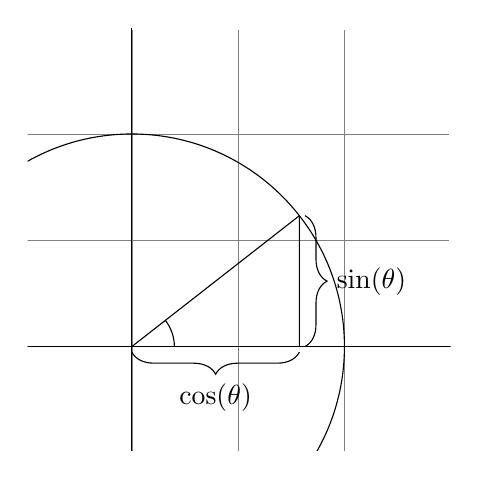
\begin{tikzpicture}[scale=2.7]
	\clip (1.5,1.5) rectangle (-0.49,-0.49);

	\coordinate (O) at (0,0);
	\coordinate (P) at (38:1);
	\coordinate (I) at (P |- O);

	\draw [step=0.5, gray, ultra thin] (1.49,1.49) grid (-1.49,-1.49);

	\draw (-1.5,0) -- (1.5,0) (0,1.5) -- (0,-1.5);
	\draw (0,0) circle[radius=1];

	\draw (0,0) -- (P);
	\draw (P) -- (I);

	\draw (0.2,0) arc[start angle=0, end angle=38, radius=0.2];
	%\draw (0.1,0) node [anchor=south west] {$\theta$};

	\draw [decorate, decoration={brace, amplitude=8pt, raise=2pt}] (P) -- node [right, xshift=10pt] {$\sin(\theta)$} (I);
	\draw [decorate, decoration={brace, amplitude=8pt, mirror, raise=2pt}] (O) -- node [below, yshift=-10pt] {$\cos(\theta)$} (I);
\end{tikzpicture}
}\end{minipage}\hspace{3ex}
\begin{minipage}{0.25\linewidth}
	\large
	$$\tan\theta = \frac{\sin\theta}{\cos\theta}$$
	\vspace{1em}
	$$\sec\theta = \frac{1}{\cos\theta}$$
	\vspace{1em}
	$$\cosec\theta = \frac{1}{\sin\theta}$$
	\vspace{1em}
	$$\cot\theta = \frac{1}{\tan\theta} = \frac{\cos\theta}{\sin\theta}$$
\end{minipage}
\end{figure}

\vspace{3em}

\sectitle{Identities}

\begin{figure}[h]
\centering
\large
\begin{minipage}{0.3\linewidth}
	$$\sin^2\theta + \cos^2\theta \equiv 1$$
\end{minipage}\hfill
\begin{minipage}{0.3\linewidth}
	$$1 + \tan^2\theta \equiv \sec^2\theta$$
\end{minipage}\hfill
\begin{minipage}{0.3\linewidth}
	$$1 + \cot^2\theta \equiv \cosec^2\theta$$
\end{minipage}
\normalsize
\end{figure}

\begin{figure}[h]
\centering
\large
\begin{minipage}{0.49\linewidth}
	$$\sin(\alpha + \beta) \equiv \sin\alpha\cos\beta + \cos\alpha\sin\beta$$
	\vspace{0.5em}
	$$\cos(\alpha + \beta) \equiv \cos\alpha\cos\beta - \sin\alpha\sin\beta$$
	\vspace{0.5em}
	$$\tan(\alpha + \beta) \equiv \frac{\tan\alpha + \tan\beta}{1 - \tan\alpha\tan\beta}$$
\end{minipage}\hfill
\begin{minipage}{0.49\linewidth}
	$$\sin(\alpha - \beta) \equiv \sin\alpha\cos\beta - \cos\alpha\sin\beta$$
	\vspace{0.5em}
	$$\cos(\alpha - \beta) \equiv \cos\alpha\cos\beta + \sin\alpha\sin\beta$$
	\vspace{0.5em}
	$$\tan(\alpha - \beta) \equiv \frac{\tan\alpha - \tan\beta}{1 + \tan\alpha\tan\beta}$$
\end{minipage}
\normalsize
\end{figure}

\begin{figure}[H]
\centering
\large
\begin{minipage}{0.49\linewidth}
$$\sin 2\theta \equiv 2\sin\theta\cos\theta$$
\vspace{0.5em}
$$\tan2\theta \equiv \frac{2\tan\theta}{1 - \tan^2\theta}$$
\end{minipage}\hfill
\begin{minipage}{0.49\linewidth}
$$\cos 2\theta \equiv \cos^2\theta - \sin^2\theta$$
$$\equiv 2\cos^2\theta - 1$$
$$\equiv 1 - 2\sin^2\theta$$
\end{minipage}
\normalsize
\end{figure}

\newpage

\sectitle{Calculus}

\begin{figure}[h]
\centering
\large
\begin{minipage}{0.49\linewidth}
	$$\diff{x}\sin x = \cos x$$
	\vspace{0.5em}
	$$\diff{x}\cos x = -\sin x$$
	\vspace{0.5em}
	$$\diff{x}\tan x = \sec^2 x$$
	\vspace{0.5em}
	$$\diff{x}\sec x = \sec x\tan x$$
	\vspace{0.5em}
	$$\diff{x}\cosec x = -\cosec x\cot x$$
	\vspace{0.5em}
	$$\diff{x}\cot x = -\cosec^2 x$$
\end{minipage}\hfill
\begin{minipage}{0.49\linewidth}
	$$\inte{\sin x}{x} = -\cos x + C$$
	\vspace{0.5em}
	$$\inte{\cos x}{x} = \sin x + C$$
	\vspace{0.5em}
	$$\inte{\tan x}{x} = \ln|\sec x|+ C$$
	\vspace{0.5em}
	$$\inte{\sec x}{x} = \ln|\tan x + \sec x| + C$$
	\vspace{0.5em}
	$$\inte{\cosec x}{x} = -\ln|\cot x + \cosec x| + C$$
	\vspace{0.5em}
	$$\inte{\cot x}{x} = \ln|\sin x| + C$$
\end{minipage}
\end{figure}

\newpage

\vspace{-2.5em}

\sectitle{Graphs}

\vspace{-1em}

\begin{center}
\begin{figure}[H]
\centering
\begin{minipage}{0.5\linewidth}
	\begin{tikzpicture}
		\begin{axis}[sin cos axis]
			\addplot [trig plot] {sin(deg(x))};
			\coordinate (title) at (axis cs:0,1.2) {};
		\end{axis}

		\node at (title) [above] {$y = \sin(x)$};
	\end{tikzpicture}
\end{minipage}\hfill
\begin{minipage}{0.5\linewidth}
	\begin{tikzpicture}
		\begin{axis}[vertical asymptote axis]
			\addplot [trig plot] {1/sin(deg(x))};

			\verticalAsymptote{-6.2832}
			\verticalAsymptote{-3.1416}
			\verticalAsymptote{0}
			\verticalAsymptote{3.1416}
			\verticalAsymptote{6.2832}

			\coordinate (title) at (axis cs:0,4.2) {};
		\end{axis}

		\node at (title) [above] {$y = \cosec(x)$};
	\end{tikzpicture}
\end{minipage}
\end{figure}

\begin{figure}[H]
\centering
\begin{minipage}{0.5\linewidth}
	\begin{tikzpicture}
		\begin{axis}[sin cos axis]
			\addplot [trig plot] {cos(deg(x))};
			\coordinate (title) at (axis cs:0,1.2) {};
		\end{axis}

		\node at (title) [above] {$y = \cos(x)$};
	\end{tikzpicture}
\end{minipage}\hfill
\begin{minipage}{0.5\linewidth}
	\begin{tikzpicture}
		\begin{axis}[vertical asymptote axis]
			\addplot [trig plot] {1/cos(deg(x))};

			\verticalAsymptote{-4.7124}
			\verticalAsymptote{-1.5708}
			\verticalAsymptote{1.5708}
			\verticalAsymptote{4.7124}

			\coordinate (title) at (axis cs:0,4.2) {};
		\end{axis}

		\node at (title) [above] {$y = \sec(x)$};
	\end{tikzpicture}
\end{minipage}
\end{figure}

\begin{figure}[H]
\centering
\begin{minipage}{0.5\linewidth}
	\begin{tikzpicture}
		\begin{axis}[vertical asymptote axis]
			\addplot [trig plot] {tan(deg(x))};

			\verticalAsymptote{-4.7124}
			\verticalAsymptote{-1.5708}
			\verticalAsymptote{1.5708}
			\verticalAsymptote{4.7124}

			\coordinate (title) at (axis cs:0,4.2) {};
		\end{axis}

		\node at (title) [above] {$y = \tan(x)$};
	\end{tikzpicture}
\end{minipage}\hfill
\begin{minipage}{0.5\linewidth}
	\begin{tikzpicture}
		\begin{axis}[vertical asymptote axis]
			\addplot [trig plot] {1/tan(deg(x))};

			\verticalAsymptote{-6.2832}
			\verticalAsymptote{-3.1416}
			\verticalAsymptote{0}
			\verticalAsymptote{3.1416}
			\verticalAsymptote{6.2832}

			\coordinate (title) at (axis cs:0,4.2) {};
		\end{axis}

		\node at (title) [above] {$y = \cot(x)$};
	\end{tikzpicture}
\end{minipage}
\end{figure}
\end{center}

\end{document}
